\chapter{Continental}
	\section{Organisation de l'entreprise}
		\subsection{Continental AG}
		Continental AG est une entreprise allemande dont le siège principal est à Hanovre. Il s'agit d'une Société Anonyme dont le président du comité de direction est depuis le 11 septembre 2001 Manfred Wennemer. Plus de 170.000 collaborateurs qui sont employés dans plus de 200 sites dans 45 pays appartenant à l'entreprise. En Allemagne Continental est une S.A. numéro un du marché de Production de pneu toutefois il s'agit aussi d'un équipementier automobile important. 

		Continental AG a été fondée en 1871 et est à nouveau membre depuis août 2003 de DAX. En 2007 elle a obtenu un chiffre d'affaires de 16 milliards d'Euros. L'entreprise est composée de 2 grands groupes auxquels sont rattachées 6 branches\footnote{cf figure \ref{fig:structConti}}.
		 
		 \begin{figure}[H]
		 	\centering
		 	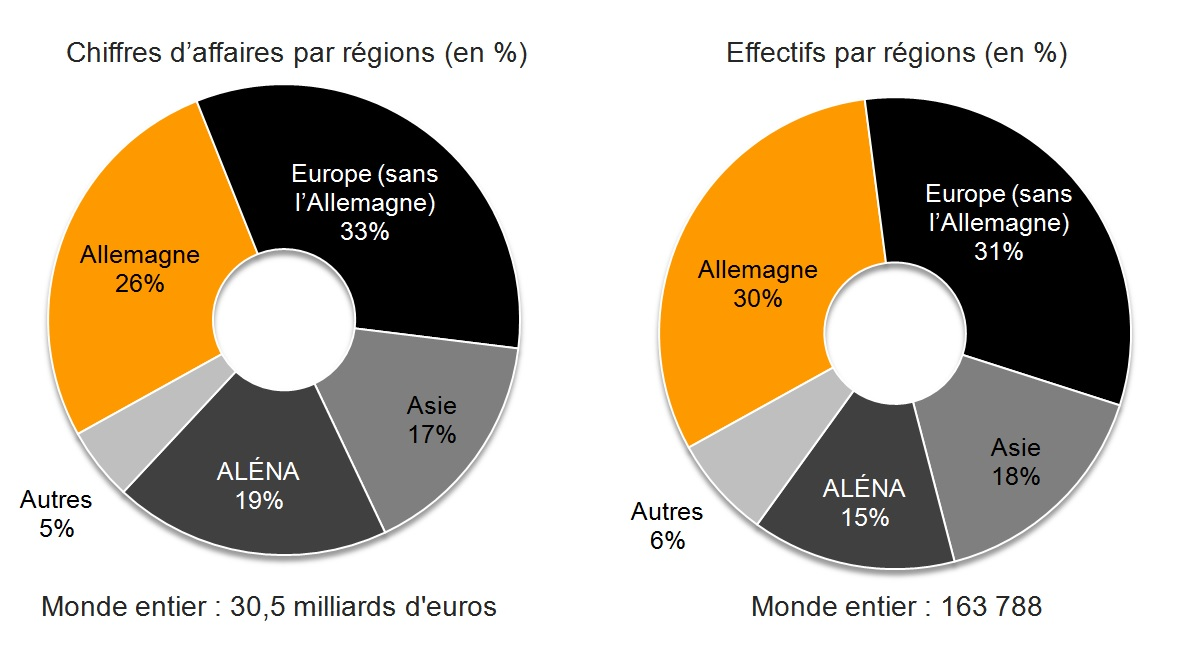
\includegraphics[width=12cm]{contents/images/caConti.jpg}
		 	\caption{Chiffre d'affaire et nombre d'employés}
		 	\label{fig:caConti}
		 \end{figure}

		 L'entreprise compte plus de $163000$ employés dans le monde répartis dans 269 sites et 46 pays différents comme le montre la figure \ref{fig:repartitionConti}. (Chiffres 2011)
		 \begin{figure}[H]
		 	\centering
		 	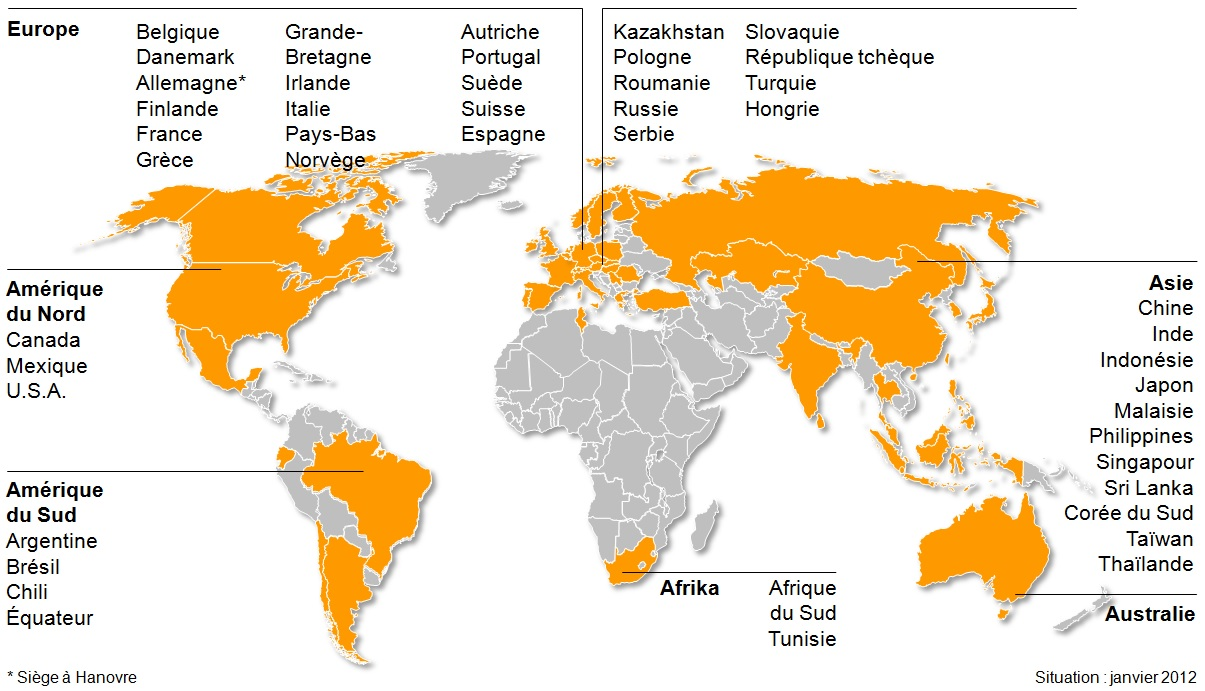
\includegraphics[width=13cm]{contents/images/repartitionConti.jpg}
		 	\caption{Répartition du groupe continental dans le monde}
		 	\label{fig:repartitionConti}
		 \end{figure}		 

		\subsection{Histoire de l'entreprise}
		Continental est fondée en 1871 comme société anonyme sous le nom de <<Continental-Caoutchouc-und Gutta-Percha Compagnie>> par neuf banquiers et industriels de Hanovre (Allemagne).

		Continental dépose l'emblème du cheval comme marque de fabrique à l'Office impérial des brevets de Hanovre en octobre 1882. Il est aujourd'hui encore protégé en tant que marque distinctive.
		\begin{figure}[H]
			\centering
			
\includegraphics[width=2cm]{contents/images/logo.jpg}
			\caption{Logo de Continental}
			\label{fig:logo}
		\end{figure}

		Le fabricant de pneus allemand débute son expansion à l'international en tant que sous-traitant automobile international en 1979, expansion qu'il n'a cessé de poursuivre depuis de manière systématique.
		
		Entre 1979 et 1985 Continental pose définitivement un pied en Europe avec le rachat l'acquisition des activités pneumatiques européennes de l'américain Uniroyal Inc. Et de la marque de pneus autrichienne Semperit.

		En 1995 est créée la Division Automotive Systems pour intensifier les activités <<systèmes>> avec l'industrie automobile.

		Pour renforcer sa position sur les marchés américain et asiatique, Continental fait l'acquisition en 2001 du spécialiste international de l'électronique Temic, qui dispose de sites de production en Amérique et en Asie. Deux autres reprises ont lieu en 2001. Continental reprend la majorité des parts de deux entreprises japonaises produisant des composants d'actionnement des freins et des freins à disques.

		En 2004, le plus grand spécialiste mondial de la technologie du caoutchouc et des plastiques naît de la fusion entre Phoenix AG et ContiTech.

		En juillet 2007 Continental réalise son plus gros rachat sur le fournisseur automobile Siemens VDO Automotive, ce rachat à permis à l'entreprise de multiplier son chiffre d'affaire par deux : de 13 à plus de 30 milliards d'euros (chiffre 2011). 

		% \begin{figure}[H]
		% 	\centering
		% 	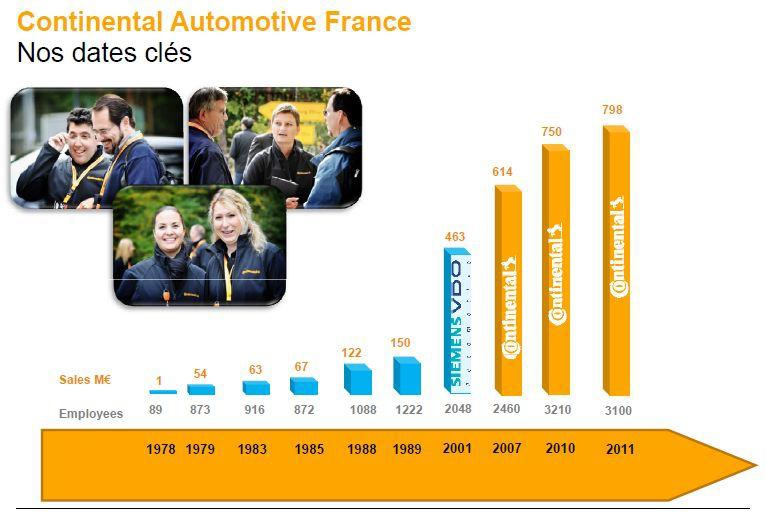
\includegraphics[width=14cm]{contents/images/datesCles.jpg}
		% 	\caption{Dates clés}
		% 	\label{fig:datesCles}
		% \end{figure}
		
		\subsection{Activités des différentes branches}
		\begin{figure}[H]
			\centering
			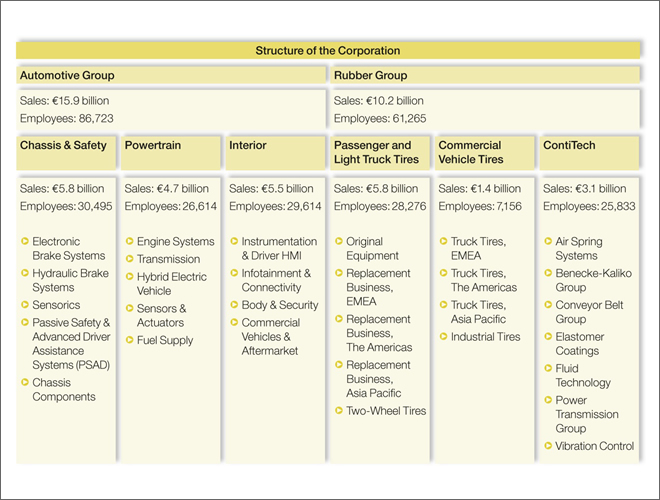
\includegraphics[width=18cm]{contents/images/structureConti.jpg}
			\caption{Structure de continental}
			\label{fig:structConti}
		\end{figure}

		Comme on peut le voir sur la figure \ref{fig:structConti}, le groupe est constitué de 6 divisions. Ces divisions sont ensuite divisées en Business Units qui ont une activité bien particulière dans leur domaine de compétence. Elles se chargent de développer et produire des équipements répondant aux besoins de nos clients.

Durant ce stage, j'étais dans la division \textit{powertrain}. Celle-ci s'occupe essentiellement du contrôle moteur, au niveau logiciel, materiel avec l'ECU\footnote{Engine Control Unit}, mise au point et des systèmes diesel et essence.

Par exemple, la Business Unit <<Engine Systems>> est chargée de produire les équipements nécessaires au contrôle moteur tels que des calculateurs ou des 
injecteurs.

	\section{Le contexte de l'équipe Vérification \& Validation}
		\subsection{L'équipe}
		J'ai travaillé dans l'équipe en charge de la vérification et de la validation des logiciels.\footnote{Plus précisément dans le service P-ES-E-SYS-ETV-V.\newline P: Powertrain\newline ES-E-SYS: Engine Systems\newline ETV: Engineering Tool and Verification\newline V: Vérification.}
		Cette équipe est en charge du développement, de la configuration et de l'exécution de scripts de Tests sur bancs HIL\footnote{Hardware in the Loop}, pour les tests de régression automatiques\footnote{Aussi appelés FaST : Functions and Software Testing}, avant la livraison des projets.
		
		\subsection{Le besoin} \label{besoinTests}
		Le contrôle moteur d'une voiture est un dispositif très important et à haut risque, en effet une défaillance peut provoquer la mort de plusieurs personnes. Ainsi, le test est indispensable dans ce domaine, et doit être robuste. Le test est ainsi une très grande partie du cycle de vie.\newline
		 Il est donc nécessaire d'éviter le maximum d'erreurs possibles dans les logiciels. Un logiciel ne peut pas comporter aucun bug, il est cependant possible d'éviter le maximum de bugs critiques et d'erreurs. Pour cela, il est nécessaire d'automatiser cette vérification, afin d'éviter les erreurs humaines due à l'innatention ou la répétition de.\\
		De plus, un contrôle moteur possède un très grand nombre de cas de tests, il serait impensable de tout tester << à la main >>.

		C'est dans ce contexte que l'équipe Vérification \& Validation intervient, elle doit fournir des outils aux développeurs afin de vérifier facilement et correctement leur travail, particulièrement pour des tests de régression, bien que l'outil que l'équipe est en train de développer est à destination de tests d'intégration.

